\documentclass[a4wide,11pt]{article}

\usepackage{amsmath}
\usepackage{amssymb}
\usepackage{graphicx}
\usepackage{siunitx}
\usepackage[linkcolor = blue, citecolor = blue, urlcolor = blue, colorlinks = true]{hyperref}
\usepackage[capitalise]{cleveref}
\usepackage{commath}
\usepackage{tabu}
\usepackage{booktabs}
\usepackage[T1]{fontenc}
\usepackage[protrusion = true, expansion = true]{microtype}
\usepackage{subdepth}

\begin{document}

\title{Summary of chemotaxis in porous media}
\author{Elliot Marsden}
\date{July 2014}
\maketitle

\tableofcontents
\newpage

\section{Diffusion of active particles in a continuous environment}

We investigate two types of active particle: Active Brownian Particles (\textsc{abp}s), whose direction diffuses slowly with rotational diffusion constant $\mathrm{D}_r$, and Run and Tumble Particles (\textsc{rtp}s), whose direction is completely randomised at a uniform rate $\alpha$. Over long time intervals, the free-space diffusivity of the two particles is the same (\cref{free_D}).

\begin{figure}
    \centering
    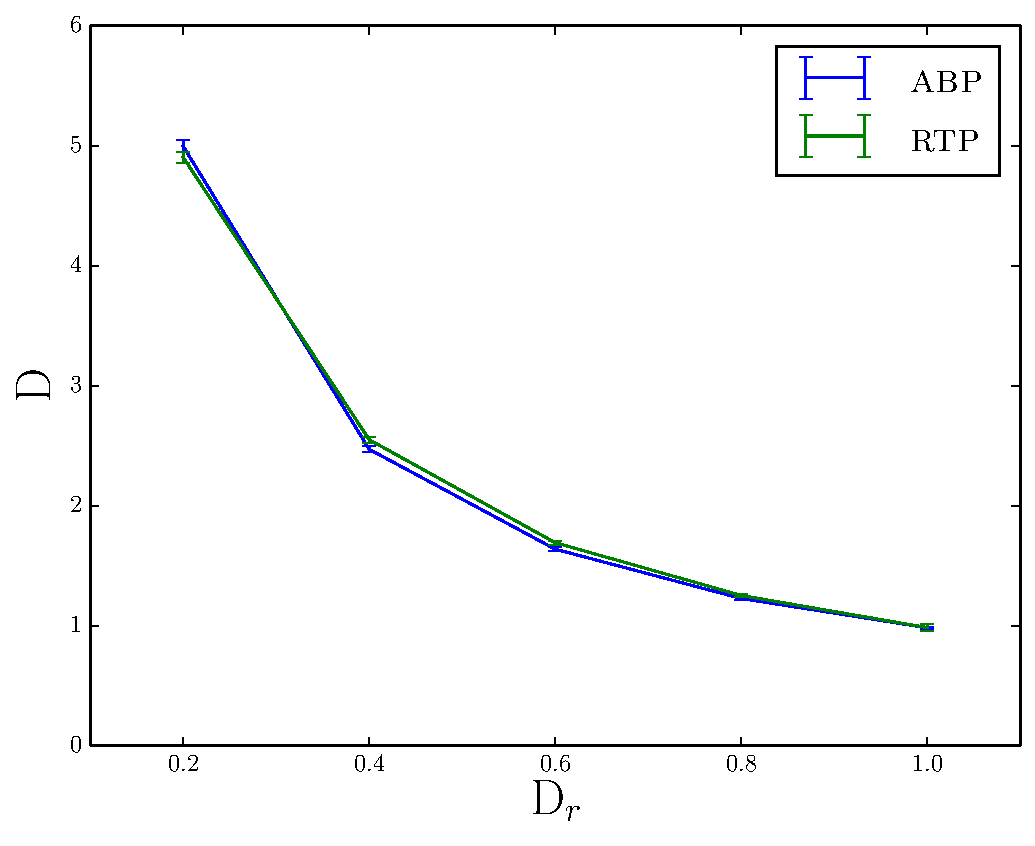
\includegraphics[width=0.7\textwidth]{img/free_space_D_of_Dr.pdf}
    \caption{Diffusivity of active particles in free space as a function of the effective rotational diffusion constant. For \textsc{rtp}s, $\alpha$ is equivalent to $\mathrm{D}_r$ over long time intervals.}
    \label{free_D}
\end{figure}

\section{Drift of chemotactic active particles in a continuous environment}

We allow for chemotaxis in the dynamics of both particle types by first introducing a measure, the `chemotactic fitness' of a particle trajectory, $f(\mathbf{v}(t), c(t))$, where $c(t)$ is the chemical concentration at the particle's position at time $t$.

Secondly, we vary the strength of the particle's rotational noise according to $f$: for \textsc{abp}s, $\mathrm{D}_r = \mathrm{D}_r(f)$ (for \textsc{rtp}s replace $\mathrm{D}_r$ with the tumbling rate $\alpha$). We choose a linear response for $\mathrm{D}_r$:

\begin{equation}
    \mathrm{D}_r(f) = \mathrm{D}_{r,0} (1 - f)
    \label{Dr}
\end{equation}

where $\mathrm{D}_{r,0}$ is the free-space rotational diffusion constant.

We investigate two forms for $f$. The first is proportional to the instantaneous degree of alignment between the particle's direction and the chemical gradient, 

\begin{equation}
    \begin{aligned}
        f_s &= \chi \dfrac{\dot{c}}{\mathrm{v}} \,, \\
        \dot{c} &= \mathbf{v}(t) \cdot \nabla c(t) \,,
    \end{aligned}
    \label{f_s}
\end{equation}

where $\chi$ controls the strength of the chemotactic response. $\dot{c}$ represents the time-derivative of the chemical concentration in the particle's reference frame. The second form is a time-averaged approximation of the first:

\begin{equation}
    \begin{aligned}
        f_t &= \chi \dfrac{\tilde{\dot{c}}}{\mathrm{v}} \,, \\
        \tilde{\dot{c}} &= \mathrm{N} \int_0^t K(t - t') c(t') \dif t' \,,
    \end{aligned}
    \label{f_t}
\end{equation}

where $K$ is a kernel which acts to transform the particle's measured chemical concentration history into an approximate co-moving chemical concentration change, and $\mathrm{N}$ is a normalisation constant. $\mathrm{N}$ is chosen such that a particle moving directly up a constant chemical gradient with no rotational noise, gives the same value for $f_s$ and $f_t$ (see Appendix A).

We refer to particles using $f_s$ as doing `spatial chemotaxis', and those using $f_t$ as doing `temporal chemotaxis'.

We investigate the behaviour of these particle in an environment with a chemical gradient that is constant in time and space, of magnitude $1$ in the direction $\hat{\mathbf{u}}_c$. The effectiveness of chemotaxis is measured by the drift speed in the direction of the gradient, $\mathrm{v}_d = \langle \mathbf{v} \cdot \nabla \mathbf{c} \rangle$. \Cref{free_chi} shows the effect of changing the strength of chemotaxis on the drift speed, alongside a comparison with theoretical predictions for \textsc{abp}s (see Appendix B). For spatial chemotaxis, \textsc{abp}s and \textsc{rtp}s have identical drift speeds. For temporal chemotaxis, this equivalence breaks down: \textsc{rtp}s do temporal chemotaxis more effectively than \textsc{abp}s.

\begin{figure}
    \centering
    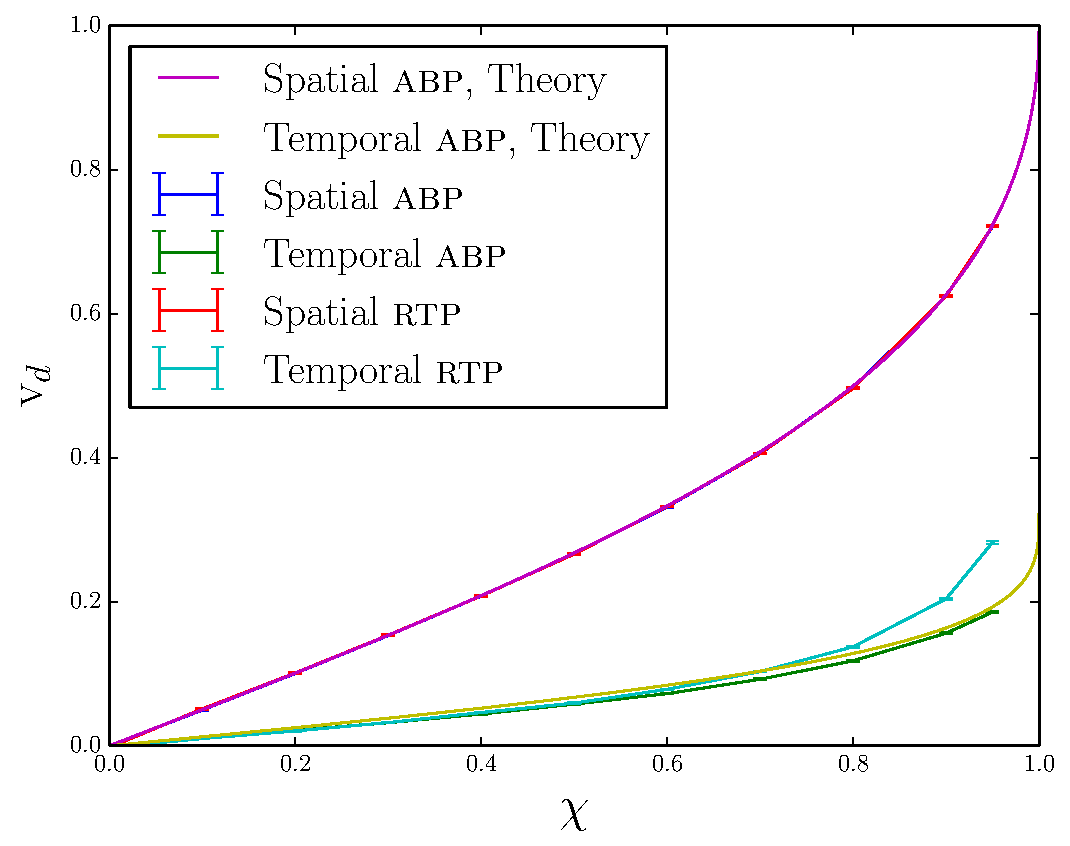
\includegraphics[width=0.7\textwidth]{img/free_space_vd_of_chi.pdf}
    \caption{The dependence of the drift speed of \textsc{abp}s and \textsc{rtp}s in free space, on the chemotaxis strength parameter, $\chi$, for `spatial' and `temporal' chemotaxis. The two `spatial' curves lie on top of one another. Also shown are theoretical predictions for both \textsc{abp} curves.}
    \label{free_chi}
\end{figure}

\section{Diffusion of active particles in a porous environment}

We now look at the behaviour of non-chemotactic active particles in porous environments formed by randomly placed non-overlapping circles of a constant radius, up to some packing fraction, $\phi$. A particle colliding with such an obstacle reverses its velocity component perpendicular to the obstacle surface (that is, it bounces off the obstacle).

\Cref{D_of_packing} shows the effect of obstructing \textsc{abp}s on how fast they diffuse through the environment. As expected, higher packing fractions cause the particles to diffuse more slowly. In free space, reducing the amount of rotational noise always increases the diffusivity, however in a porous medium this is no longer strictly true, as can be seen in \cref{packed_D_of_Dr}. A very low amount of rotational noise means the particles collide with the environment frequently, so some noise is useful in helping the particles navigate through the environment.

\begin{figure}
    \centering
    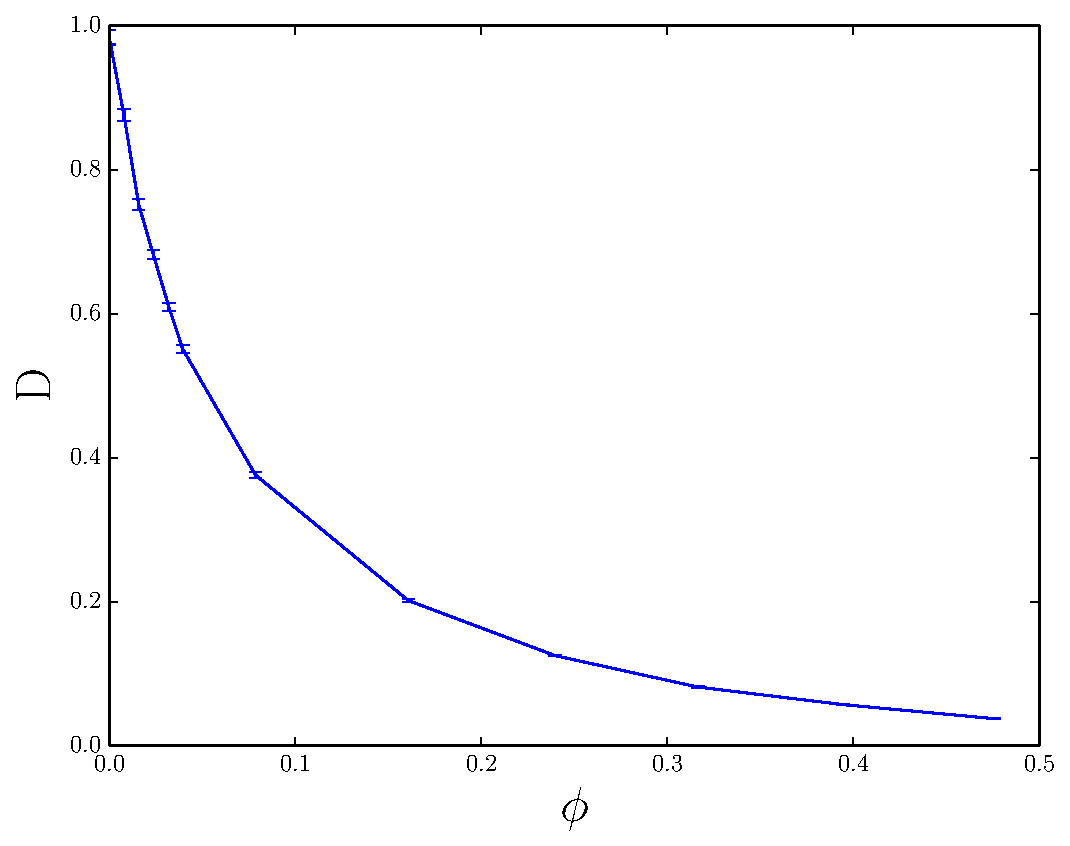
\includegraphics[width=0.7\textwidth]{img/D_of_packing.pdf}
    \caption{The diffusivity of \textsc{abp}s in a porous medium as a function of the packing fraction.}
    \label{D_of_packing}
\end{figure}

\begin{figure}
    \centering
    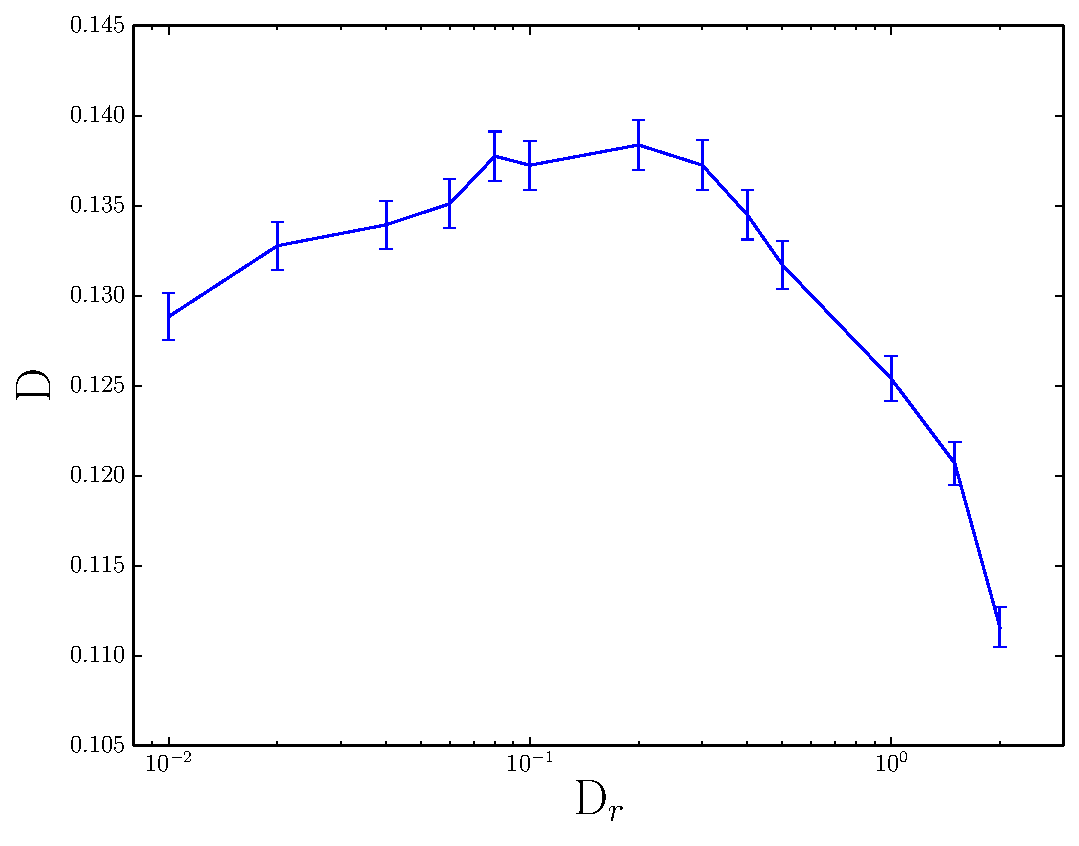
\includegraphics[width=0.7\textwidth]{img/packed_D_of_Dr.pdf}
    \caption{The dependence of the diffusivity of \textsc{abp}s in a porous medium, with constant packing fraction $\phi=24\%$, on the rotational diffusion constant.}
    \label{packed_D_of_Dr}
\end{figure}

\section{Drift of chemotactic active particles in a porous environment}

For `spatial' and `temporal' chemotaxis with \textsc{abp}s, we choose $\chi$ for both such that the free-space drift speeds are identical, and investigate how effective chemotaxis is as the packing fraction changes. \Cref{vd_of_packing} shows that particles doing spatial chemotaxis are more effective than those doing temporal chemotaxis in the same environment. This is presumably due to collisions with obstacles disrupting the time averaging being done in the latter case.

\begin{figure}
    \centering
    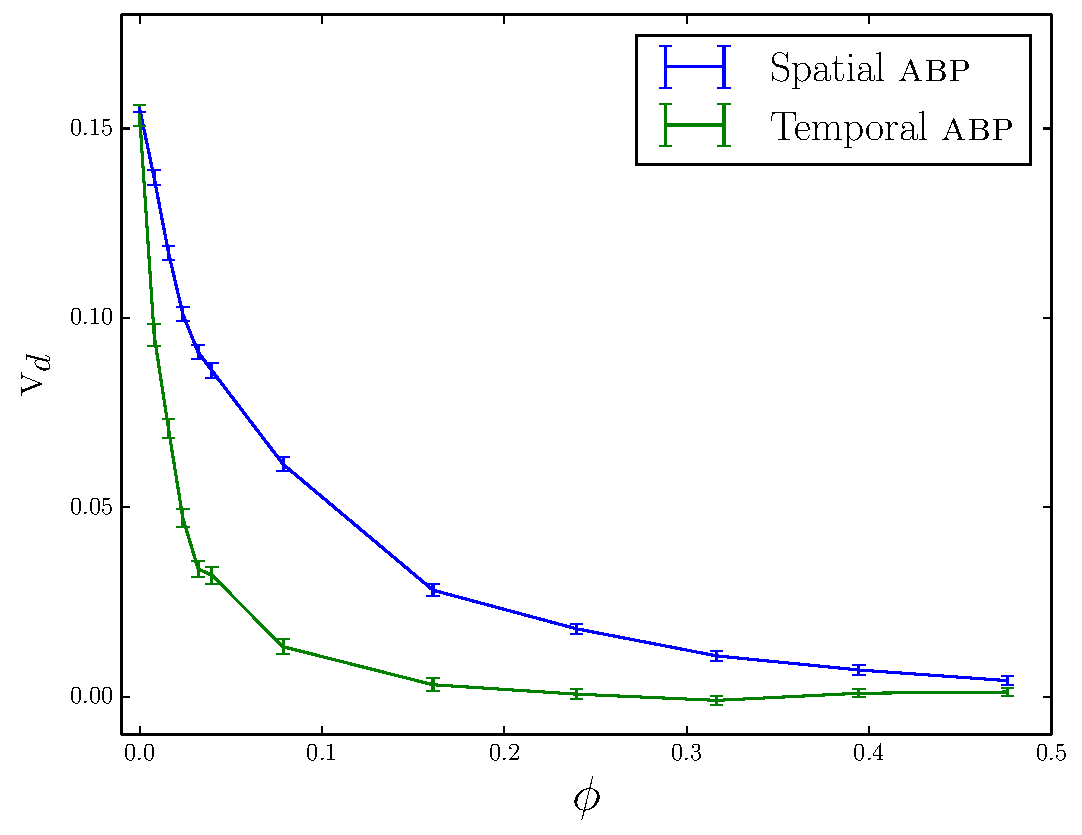
\includegraphics[width=0.7\textwidth]{img/vd_of_packing.pdf}
    \caption{The dependence of the drift speed of \textsc{abp}s in a porous medium, on the packing fraction, for `spatial' and `temporal' chemotaxis. For spatial chemotaxis, $\chi=0.304$ was used, and for temporal $\chi=0.9$; chosen such that the free-space drift speeds are identical.}
    \label{vd_of_packing}
\end{figure}

\begin{table}
    \centering
    \begin{tabu} to \linewidth {lll}
        \toprule
        Parameter & Label & Value \\
        \midrule
        Dimension & $\mathrm{d}$ & $2$ \\
        System size & $\mathrm{L}$ & $1$ \\
        Time-step & $\dif t$ & $0.001$ \\
        Number of particles & $\mathrm{n}$ & $10^4$ \\
        Particle speed & $\mathrm{v}$ & $1$ \\
        Base rotational diffusion constant & $\mathrm{D}_{r,0}$ & $1$ \\
        Base tumble rate & $\alpha_0$ & $1$ \\
        Obstacle radius & $\mathrm{R}$ & $0.05$ \\
        \bottomrule
    \end{tabu}
    \caption{Parameters used in all simulations, except where indicated otherwise.}
\end{table}

\section*{Appendix A: Normalisation of temporal chemotaxis integral}
\addcontentsline{toc}{section}{Appendix A: Normalisation of temporal chemotaxis integral}

\subsection*{Maximum fitness of spatial chemotaxis}

Assume a chemical gradient constant in time and space, of magnitude $1$, in direction $\hat{\mathbf{u}}_c$. From \cref{f_s},


\begin{equation}
    \begin{aligned}
        f_s     &= \chi \dfrac{\dot{c}}{\mathrm{v}} \,, \\
        \dot{c} &= \mathbf{v}(t) \cdot \hat{\mathbf{u}}_c \\
                &= \mathrm{v} \cos \theta \,.
    \end{aligned}
    \label{f_s_uni}
\end{equation}

Clearly then the maximum fitness is when $\theta = 0$, that is, when the particle moves directly up the concentration gradient. In this case, $\dot{c} = \mathrm{v}$, and $f_s = \chi$.

\subsection*{Calibrating temporal chemotaxis}

We want the maximum fitness to be the same for spatial and temporal chemotaxis. From \cref{f_t} we can see that this requires $f_{t,\mathrm{max}} = \chi$, and thus $\tilde{\dot{c}}_\mathrm{max} = \mathrm{v}$.

We assume that the fitness is again maximised when the particle moves directly up the chemical gradient, $\mathbf{v} = \mathrm{v} \hat{\mathbf{u}}_c$. This means that the chemical concentration at the particle's position at time $t$ is,

\begin{equation}
    \begin{aligned}
        c(t) &= c(0) + (\mathbf{v} \cdot \hat{\mathbf{u}}_c) t \\
             &= c(0) + \mathrm{v} t \,.
    \end{aligned}
    \label{c_direct}
\end{equation}

Substituting \cref{c_direct} into \cref{f_t},

\begin{equation}
    \begin{aligned}
        \tilde{\dot{c}} &= \mathrm{N} \int_0^t K(t - t') \del{ c(0) + \mathrm{v} t' } \dif t' \\
                        &= \mathrm{N} \del{ c(0) \int_0^t K(t - t') \dif t' + \mathrm{v} \int_0^t K(t - t') t' \dif t' } \,.
    \end{aligned}
    \label{f_t_uni}
\end{equation}

The particular form we use for $K$ is

\begin{equation}
    K(t) = \exp(-t) \del{1 - \dfrac{t}{2} - \dfrac{t^2}{4}} \,
    \label{K}
\end{equation}

Assuming the particle points up the chemical gradient for a sufficiently long time, we can take $t \to \infty$. Computing the first integral in this limit gives

\begin{equation}
    \begin{aligned}
        \int_0^\infty K(-t) \dif t &= \left[ \dfrac{1}{4} \exp(-t) t \del{t + 4} \right]_0^\infty \\
                                  &= 0 \,.
    \end{aligned}
    \label{term1}
\end{equation}

This means that the first term in \cref{f_t_uni} vanishes. Computing the second integral in the same limit,

\begin{equation}
    \begin{aligned}
        \int_0^\infty t K(-t) \dif t &= \left[ \dfrac{1}{4} \exp(-t) \del{t \del{t + 2} \del{t + 3} + 6} \ \right]_0^\infty \\
                                    &= \dfrac{3}{2} \,.
    \end{aligned}
    \label{term2}
\end{equation}

So using~\cref{term1,term2} in~\cref{f_t_uni},

\begin{equation}
    \tilde{\dot{c}} = \dfrac{3}{2} \mathrm{N} \mathrm{v} \,.
    \label{f_t_uni_subsed}
\end{equation}

This means that for our spatial and temporal chemotaxis forms to be comparable, $\mathrm{N} = \dfrac{2}{3}$.

\section*{Appendix B: Derivation of expression for drift speed of \textsc{abp}s doing spatial chemotaxis}
\addcontentsline{toc}{section}{Appendix B: Derivation of expression for drift speed of \textsc{abp}s doing spatial chemotaxis}

Assume an environment with a chemical gradient that is constant in time and space, of magnitude $1$in the direction $\hat{\mathbf{u}}_c$. Take $\theta$ to be the angle between this and the particle's velocity. A particle swimming with orientation $\theta$ has a drift speed $\mathrm{v}_d = \mathrm{v} \cos \theta$. Over long times, assuming the particle ergodically samples all $\theta$ (meaning that $\mathrm{D}_r > 0$ at all times), then the particle has an average drift speed,

\begin{equation}
    \begin{aligned}
        \mathrm{v}_d &= \int_{-\pi}^{\pi} P(\theta) \mathrm{v}_d(\theta) \dif \theta \\
                  &= \mathrm{v} \int_{-\pi}^{\pi} P(\theta) \cos \theta \dif \theta \,,
    \end{aligned}
    \label{drift_master}
\end{equation}

where $P(\theta)$ is the probability of the particle being at orientation $\theta$.

From simulations, for spatial chemotaxis we find that $P(\theta) \propto \dfrac{1}{\mathrm{D}_r(\theta)}$. This means that,

\begin{equation}
    P(\theta) = \dfrac{\mathrm{D}_r(\theta)^{-1}}{\int_{-\pi}^{\pi} \mathrm{D}_r(\theta)^{-1} \dif \theta} \,.
    \label{P}
\end{equation}

\subsection*{Calculating the normalisation constant}

Substituting \cref{f_s} into \cref{Dr},

\begin{equation}
    \begin{aligned}
        \mathrm{D}_r(\theta) &= \mathrm{D}_{r,0} \del{1 - f_s} \\
                    &= \mathrm{D}_{r,0} \del{1 - \chi \dfrac{\dot{c}}{\mathrm{v}}} \\
                    &= \mathrm{D}_{r,0} \del{1 - \chi \dfrac{\mathbf{v}(t) \cdot \hat{\mathbf{u}}_c}{\mathrm{v}}} \\
                    &= \mathrm{D}_{r,0} \del{1 - \chi \cos\theta} \\
    \end{aligned}
    \label{Dr_s}
\end{equation}

\begin{equation}
    \begin{aligned}
       I :&= \int_{-\pi}^{\pi} \mathrm{D}_r(\theta)^{-1} \dif \theta \\
          &= \dfrac{1}{\mathrm{D}_{r,0}} \int_{-\pi}^\pi \dfrac{\dif \theta}{1 - \chi \cos \theta} \\
          &= -\dfrac{1}{\mathrm{D}_{r,0}} \left[ \dfrac{2}{\sqrt{\chi^2 - 1}} \tanh^{-1} \del{ \dfrac{\del{\chi + 1} \tan \del{\dfrac{\theta}{2}}}{\sqrt{\chi^2 - 1}} } \right]_{-\pi}^\pi \\
    \end{aligned}
    \label{I_norm}
\end{equation}

Using the fact that $\tanh^{-1}$ and $\tan$ are odd functions,

\begin{equation}
    I = -\dfrac{1}{\mathrm{D}_{r,0}} \dfrac{4}{\sqrt{\chi^2 - 1}} \tanh^{-1} \del{ \dfrac{\del{\chi + 1} \tan \del{\dfrac{\pi}{2}}}{\sqrt{\chi^2 - 1}} } \,.
\end{equation}

Given that $\tan \del{\dfrac{\pi}{2}}=\infty$, and $\tanh^{-1}(\infty) = -\dfrac{i \pi}{2}$, then

\begin{equation}
    I = \dfrac{1}{\mathrm{D}_{r,0}} \dfrac{2 \pi i}{\sqrt{\chi^2 - 1}} \,.
\end{equation}

We know that $\chi < 1$ as this is required for $\mathrm{D}_r > 0 \; \forall \; \theta$, so we can factor out $i$, finally giving the normalisation constant as

\begin{equation}
    I = \dfrac{1}{\mathrm{D}_{r,0}} \dfrac{2 \pi}{\sqrt{1 - \chi^2}} \,.
    \label{norm}
\end{equation}

\subsection*{Deriving an expression for the drift speed}

We can now calculate the actual drift speed by substituting: \cref{norm} into \cref{drift_master}:

\begin{equation}
    \begin{aligned}
        \mathrm{v}_d &= \mathrm{v} \int_{-\pi}^{\pi} P(\theta) \cos \theta \dif \theta \\
                  &= \mathrm{v} \dfrac{\sqrt{1 - \chi^2}}{2 \pi \mathrm{D}_{r,0}} \int_{-\pi}^{\pi} \dfrac{\cos \theta}{1 - \chi \cos \theta} \dif \theta \,.
    \end{aligned}
\end{equation}

Integrating this and simplifying through almost identical steps as for the normalisation constant gives,

\begin{equation}
    \mathrm{v}_d = \mathrm{v} \dfrac{1 - \sqrt{1 - \chi^2}}{\chi} \,.
    \label{vd_s}
\end{equation}

\end{document}
